\documentclass[]{elsarticle} %review=doublespace preprint=single 5p=2 column
%%% Begin My package additions %%%%%%%%%%%%%%%%%%%
\usepackage[hyphens]{url}

  \journal{NeuroImage} % Sets Journal name


\usepackage{lineno} % add
\providecommand{\tightlist}{%
  \setlength{\itemsep}{0pt}\setlength{\parskip}{0pt}}

\usepackage{graphicx}
\usepackage{booktabs} % book-quality tables
%%%%%%%%%%%%%%%% end my additions to header

\usepackage[T1]{fontenc}
\usepackage{lmodern}
\usepackage{amssymb,amsmath}
\usepackage{ifxetex,ifluatex}
\usepackage{fixltx2e} % provides \textsubscript
% use upquote if available, for straight quotes in verbatim environments
\IfFileExists{upquote.sty}{\usepackage{upquote}}{}
\ifnum 0\ifxetex 1\fi\ifluatex 1\fi=0 % if pdftex
  \usepackage[utf8]{inputenc}
\else % if luatex or xelatex
  \usepackage{fontspec}
  \ifxetex
    \usepackage{xltxtra,xunicode}
  \fi
  \defaultfontfeatures{Mapping=tex-text,Scale=MatchLowercase}
  \newcommand{\euro}{€}
\fi
% use microtype if available
\IfFileExists{microtype.sty}{\usepackage{microtype}}{}
\bibliographystyle{elsarticle-harv}
\usepackage{longtable}
\usepackage{graphicx}
% We will generate all images so they have a width \maxwidth. This means
% that they will get their normal width if they fit onto the page, but
% are scaled down if they would overflow the margins.
\makeatletter
\def\maxwidth{\ifdim\Gin@nat@width>\linewidth\linewidth
\else\Gin@nat@width\fi}
\makeatother
\let\Oldincludegraphics\includegraphics
\renewcommand{\includegraphics}[1]{\Oldincludegraphics[width=\maxwidth]{#1}}
\ifxetex
  \usepackage[setpagesize=false, % page size defined by xetex
              unicode=false, % unicode breaks when used with xetex
              xetex]{hyperref}
\else
  \usepackage[unicode=true]{hyperref}
\fi
\hypersetup{breaklinks=true,
            bookmarks=true,
            pdfauthor={},
            pdftitle={High Resolution, Unbiased CT Brain Template},
            colorlinks=false,
            urlcolor=blue,
            linkcolor=magenta,
            pdfborder={0 0 0}}
\urlstyle{same}  % don't use monospace font for urls

\setcounter{secnumdepth}{5}
% Pandoc toggle for numbering sections (defaults to be off)

\newlength{\cslhangindent}
\setlength{\cslhangindent}{1.5em}
\newenvironment{cslreferences}%
  {\setlength{\parindent}{0pt}%
  \everypar{\setlength{\hangindent}{\cslhangindent}}\ignorespaces}%
  {\par}

% Pandoc header



\begin{document}
\begin{frontmatter}

  \title{High Resolution, Unbiased CT Brain Template}
    \author[JHSPH]{John Muschelli}
   \ead{jmusche1@jhu.edu} 
      \address[JHSPH]{Johns Hopkins Bloomberg School of Public Health, Department of Biostatistics, 615 N Wolfe St, Baltimore, MD, 21205}
    
  \begin{abstract}
  Clinical imaging relies heavily on X-ray computed tomography (CT) scans for diagnosis and prognosis. Many research applications aim to perform population-level analyses, which require images to be put in the same space, usually defined by a template. We present an open-source, publicly available, high-resolution CT template. The template was created using an unbiased template creation procedure, but is still limited by the population it was derived from, an open CT data set without demographic information. We provide a basic segmentation of the cerebrospinal fluid (CSF) spaces of the image, including the ventricles. This template can be used for spatial normalization of CT scans and research applications, including deep learning.
  \end{abstract}
  
 \end{frontmatter}

\hypertarget{introduction}{%
\section{Introduction}\label{introduction}}

Many research applications of neuroimaging use magnetic resonance imaging (MRI). MRI allows researchers to study a multitude of applications and diseases, including studying healthy volunteers. Clinical imaging, however, relies heavily on X-ray computed tomography (CT) scans for diagnosis and prognosis. Studies using CT scans cannot generally recruit healthy volunteers or large non-clinical populations due to the radiation exposure and lack of substantial benefit. As such, much of head CT data is gathered from prospective clinical trials or retrospective studies based on health medical record data and hospital picture archiving and communication system (PACS). Most of this research is on patients with neuropathology, which can cause deformations of the brain, such as mass effects.

Recently, a resource of a large number of CT scans were made avaiable (Chilamkurthy et al. 2018). These scans include people with a number of pathologies, including hemorrhagic stroke and midline shifts. More importantly, this data also includes people \textbf{without pathology} with high resolution scanning. Many clinical protocols perform axial scanning with a high within-plane resolution (e.g.\(0.5\)mm x \(0.5\)mm) but lower out-of-plane resolution (e.g.~\(5\)mm). High resolution scans (out of plane resolution \(\approx 0.5\)mm) may not be collected or reconstructed as the lower resolution scans are typically those read by the clinician or radiologist for diagnosis and prognosis.

The goal of this work is to create an anatomically unbiased, high-resolution CT template of the brain. The first, and we believe the only, publicly-available CT template was released by Rorden et al. (2012). This template was created with the specific purpose of creating a template with a similar age range as those with stroke, using 30 individuals with a mean age of 65 years old. The associated toolbox released contained a high resolution (1x1x1mm\(^3\)) template, with the skull on. Subsequent releases have included skull-stripped brain templates, but only in a lower (2x2x2mm\(^3\)) space (https://github.com/neurolabusc/Clinical). Thus, we have a high-resolution template, but not of the brain only (and skull stripping the template performs marginally well), and a low-resolution template of the brain only.
We have used these templates in previous analyses, but would like a brain template that was 1) constructed using an unbiased anatomical procedure, 2) uses more patients, 3) uses high-resolution scans to achieve a higher resolution, and 4) provide an image which dimensions are easily used in deep learning frameworks.

\hypertarget{methods}{%
\subsection{Methods}\label{methods}}

\hypertarget{data}{%
\subsubsection{Data}\label{data}}

We defined a high-resolution scan as having a within-axial resolution of \(0.7\)x\(0.7\)mm or less, with full coverage of the brain. All scans were non-contrast CT scans with a soft-tissue convolution kernel.

All data was converted from DICOM files to NIfTI (Neuroimaging Informatics Technology Initiative) using \texttt{dcm2niix}

From the CQ500 data set, 222 subjects had no indication of pathology, of which 141 had a high-resolution scan (if multiple were present, the one with the highest was present). From these 141 people, 130 had thick-slice scanns where the out-of-plane resolution was greater than \(4\)mm.

We chose an image (patient CQ500CT100 from CQ500) with a resolution of \(0.488\)x\(0.488\)x\(0.5\)mm. The head was skull-stripped so that only brain tissue and CSF spaces were kept. The image was resampled to \(0.5\)mm\(^3\) resolution so that the voxels are isotropic and high resolution. As most head CT have a within-axial dimension of 512x512, we padded the image back to 512x512, and the image had 336 coronal-plane slices. This image was used for template creation. After the template was created, we padded the coronal plane so that the template was 512x512x512. The intention is that these dimensions allow it easier to create sub-sampled arrays that are cubes and multiples of 8, such as 256x256x256 or 64x64x64 with isotropic resolution. These mutliples are particularly important in certain deep learning architectures and frameworks. Thus, we believee these dimensions allow researchers to transform the head images into a standard, isotropic space that is conducive to deep learning.

The main downside with the CQ500 data set is that no demographic or clinical information was given for each patient, save for indication for pathology. Therefore, we cannot attest the general population of interest for this template. In future work, we will prepare age-specific templates for each population based on hospital scans and records. One of the
This work aims to produce a high-resolution, publicly-available template that was based on publicly-available data.

\hypertarget{template-creation}{%
\subsubsection{Template Creation}\label{template-creation}}

The process of template creation was as follows:

\begin{enumerate}
\def\labelenumi{\arabic{enumi}.}
\tightlist
\item
  Register all images to the template \(\bar{T}_{k}\) using an affine registration followed by symmetric normalization (SyN), a non-linear deformation (Avants et al. 2008). Let the transformed image be denoted as \(T_{i, k}\), where \(i\) represents subjects and \(k\) represents iteration. Let the composition of the combined affine and non-linear transformation be denoted \(G_{i, k}\). This transformation is represented by a 4D warping image. Let \(T_{1}\) be the original template chosen above and \(G_{i, 1}\) be the transformation for to the original template.
\item
  Calculate a the mean, median, and standard deviation images, where the mean image \(\bar{T}_{k} = \frac{1}{n} \sum\limits_{i = 1}^n T_{i, k}\), using a voxel-wise average.\\
\item
  Calculate the average warping transformation: \(\bar{G}_{k} = \frac{1}{n} \sum\limits_{i = 1}^n G_{i, k}\). A gradient step of \(0.2\) was set, so that
  \(\bar{T}_{k + 1} = \bar{T}_{k} \times \left(-0.2 * \bar{G}_{k}\right)\). Transform the median and standard-deviation image in the same way.
\end{enumerate}

For each iteration \(k\), we can calculate a number of measures to determine if the template has converged compared to the previous iteration \(k - 1\). We calculated the Dice Similarity Coefficient (DSC) between the mask of iteration \(k\) and \(k-1\), where the mask for iteration \(k\) is defined as \(\bar{T}_{k} > 0\). We also the Root Mean Squared Error (RMSE) of voxel intensities. The RMSE can be calculated over a series of areas, either 1) the entire image, 2) over the non-zero voxels in iteration \(k\), 3) in iteration \(k-1\), or 4) the union (or intersection) of the 2 masks. Calculation over the entire image gives an optimistic estimate as most of the image are zeroes, and the choice of either iteration \(k\) or \(k-1\) masks is arbitrary, so we calculated the RMSE over the union of the 2 masks.

To define convergence, we would like a high DSC between the masks and a low RMSE. Ideally, the convergence criteria would set a DSC of \(1\) and a RMSE less than \(1\)HU, which would indicate the voxel intensity is changing less than \(1\)HU on average. As CT scans are measured in integers, this RMSE would likely be as good as possible. We set a DSC cutoff of \(0.95\) and chose the template with the lowest RMSE. As this procedure is computationally expensive, we ran \(40\) iterations, which was adequate for achieving stable results (Figure \ref{fig:performance}).

Values of the final template that were lower than \(5\)HU were boundary regions, outside the region of the brain and likely due to singlular segmentation images, incongruent with the remainder of the image. We did not contrain the DSC and RMSE calculation excluding these regions, but excluded them from the final template.

\hypertarget{segmentation}{%
\subsubsection{Segmentation}\label{segmentation}}

Though the template itself is the main goal of the work, segmentations of the template are worthwhile in analysis. In many CT scans, the contrast between gray matter and white matter is not high, except for specific structures such as the cerebellum, corpus callosum, and basal ganglia. Separating the brain from the cerebrospinal fluid areas (mainly ventricles) are of interest in many applications. For the final template, we performed a multi-atlas segmentation using a previously published set of 35 MRI atlases (Landman et al. 2012). We registered each brain MRI with the template using SyN and applied the transformation to the associated tissue segmentation from that template. Thus, we had 35 tissue segmentations of the CT template in template space, and the segmentations were combined using STAPLE (Warfield, Zou, and Wells 2004) via the \texttt{stapler} package (Muschelli 2019).

Along with tissue-level segmentations, the atlases from Landman et al. (2012) contain 200 different structures of the brain. We have also performed the same operation, but we caution users to how well this template can provide an accurate segmentation of these structures. At least, the accuracy of the segmentation varies over tissue type, structure volume, and structure location within the brain.

\hypertarget{results}{%
\subsection{Results}\label{results}}

As we see in Figure \ref{fig:performance}A, the DSC quickly increases and reaches a high score, where the horizontal line indicates a DSC of \(0.99\). The red dot and vertical line indicate the iteration that had the maximum DSC (0.9896). As the DSC is high for all iterations past iteration \(15\), we chose the template based on the minimum RSE. In Figure \ref{fig:performance}B, we see a similar pattern of improving performance, but by lowering the RMSE. The lowest RMSE is noted by the red point with a value of \(1.47\). Thus, this iteration (iteration \(37\)) is the template we will choose.

\begin{figure}
\centering
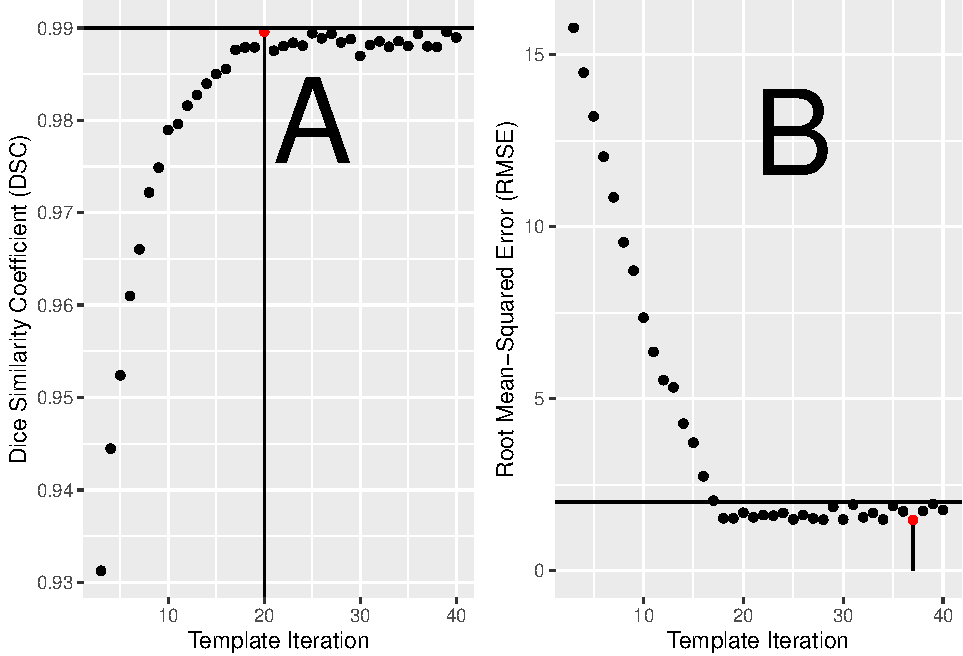
\includegraphics{index_files/figure-latex/performance-1.pdf}
\caption{\label{fig:performance}Convergence of Shape and Intensity of the Template over Iterations. Here we see the Dice Similarity Coefficient (DSC) increase between an iteration and the previous iteration, achieving high degrees of overlap, indicating the shape of the surface of the image is similar and converging (panel A). We also see the root mean-squared error (pane) drops as the iterations increase and then levels off around 4 Hounsfield units (HU), the horizontal line. The red dot indicates the iteration chosen for the template.}
\end{figure}

See Figure\ref{fig:segmentation}

\hypertarget{discussion}{%
\subsection{Discussion}\label{discussion}}

We present a high-resolution, publicly available CT template with an associated segmentation of tissues.

Though most templates are given using the mean image, we believe the standard deviation image represents variability in the area. This variability represents true systematic and biologic variability. One important area of systemic variability is registration errors. Therefore this template allows for the creation of z-score images, where a new image is registered to the mean image, the mean image is subtracted, and then divided by the standard-deviation image, so that voxels represent standard deviations away from the mean voxel.

CQ500 is Creative Commons Attribution-NonCommercial-ShareAlike 4.0 International License. Therefore, the template is released under the same license.

\hypertarget{acknowledgments}{%
\subsection{Acknowledgments}\label{acknowledgments}}

This work has been been supported by the R01NS060910 and 5U01NS080824 grants from the National Institute of Neurological Disorders and Stroke at the National Institutes of Health (NINDS/NIH).

\hypertarget{references}{%
\section*{References}\label{references}}
\addcontentsline{toc}{section}{References}

\hypertarget{supplemental-material}{%
\section{Supplemental Material}\label{supplemental-material}}

\begin{figure}
\centering
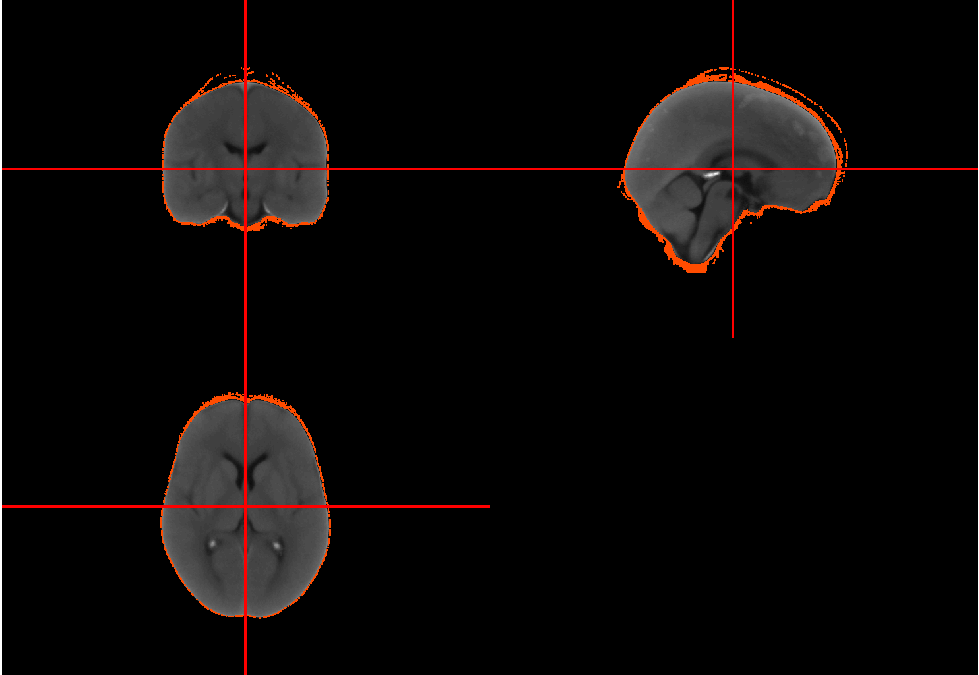
\includegraphics{index_files/figure-latex/boundary-1.pdf}
\caption{\label{fig:boundary}Boundary Issues with Low HU Values. Here we present the average image with the mask of voxels that were lower than 5HU in the template. We excluded these values from the final template.}
\end{figure}

\hypertarget{refs}{}
\begin{cslreferences}
\leavevmode\hypertarget{ref-avants_symmetric_2008}{}%
Avants, B. B., C. L. Epstein, M. Grossman, and J. C. Gee. 2008. ``Symmetric Diffeomorphic Image Registration with Cross-Correlation: Evaluating Automated Labeling of Elderly and Neurodegenerative Brain.'' \emph{Medical Image Analysis}, Special issue on the third international workshop on biomedical image registration -- WBIR 2006, 12 (1): 26--41. \url{https://doi.org/10.1016/j.media.2007.06.004}.

\leavevmode\hypertarget{ref-cq500}{}%
Chilamkurthy, Sasank, Rohit Ghosh, Swetha Tanamala, Mustafa Biviji, Norbert G Campeau, Vasantha Kumar Venugopal, Vidur Mahajan, Pooja Rao, and Prashant Warier. 2018. ``Deep Learning Algorithms for Detection of Critical Findings in Head CT Scans: A Retrospective Study.'' \emph{The Lancet} 392 (10162): 2388--96.

\leavevmode\hypertarget{ref-bennett2012miccai}{}%
Landman, Bennett Allan, Annemie Ribbens, Blake Lucas, Christos Davatzikos, Brian Avants, Christian Ledig, Da Ma, et al. 2012. \emph{MICCAI 2012 Workshop on Multi-Atlas Labeling}. CreateSpace Independent Publishing Platform.

\leavevmode\hypertarget{ref-stapler}{}%
Muschelli, John. 2019. \emph{Simultaneous Truth and Performance Level Estimation}. \url{https://CRAN.R-project.org/package=stapler}.

\leavevmode\hypertarget{ref-rorden_age-specific_2012}{}%
Rorden, Christopher, Leonardo Bonilha, Julius Fridriksson, Benjamin Bender, and Hans-Otto Karnath. 2012. ``Age-Specific CT and MRI Templates for Spatial Normalization.'' \emph{NeuroImage} 61 (4): 957--65. \url{https://doi.org/10.1016/j.neuroimage.2012.03.020}.

\leavevmode\hypertarget{ref-warfield2004simultaneous}{}%
Warfield, Simon K, Kelly H Zou, and William M Wells. 2004. ``Simultaneous Truth and Performance Level Estimation (Staple): An Algorithm for the Validation of Image Segmentation.'' \emph{IEEE Transactions on Medical Imaging} 23 (7): 903--21.
\end{cslreferences}


\end{document}

